\documentclass[10pt]{article}
\usepackage[letterpaper,hmargin=0.5in,vmargin=0.36in]{geometry}
\usepackage{longtable}
\usepackage{needspace}
\usepackage{tikz}
\usepackage{amsmath,amssymb,mathtools}
\usepackage{booktabs,array,colortbl}
\usepackage{xcolor}
\usepackage{pdfrender}
\usepackage[most]{tcolorbox}
\pagestyle{empty}
\setlength{\parindent}{0pt}
\definecolor{boxbg}{HTML}{F3F3F3}
\definecolor{boxfr}{HTML}{9A9A9A}
\definecolor{hdr}{HTML}{E4E4E4}
\newtcolorbox{sheetbox}{breakable,coltext=black,colback=boxbg,colframe=boxfr,boxrule=0.5pt,arc=2pt,left=6pt,right=6pt,top=2pt,bottom=2pt}
\newtcolorbox{smallbox}{breakable,fontupper=\small,coltext=black,colback=boxbg,colframe=boxfr,boxrule=0.5pt,arc=2pt,left=6pt,right=6pt,top=2pt,bottom=2pt}
\newcommand{\Cp}{\mathbb{C}}
\newcommand{\tr}{\operatorname{tr}}
\newcommand{\Mt}{M_2(\Cp)}
\newcommand{\eps}{\varepsilon}
\newcommand{\sinc}{\operatorname{sinc}}
\newcommand{\rep}[1]{#1}
\newcommand{\forcesline}[1]{\par\vspace{-4pt}{\centering\small\textit{(#1)}\par}\vspace{2pt}}
\newcommand{\repline}[1]{\par\vspace{-2pt}{\leftskip=0.35in\rightskip=0.2in\noindent\textbf{Group class.} #1\par}\vspace{0pt}}
\newcommand{\lean}[1]{\texttt{\detokenize{#1}}}
\newcommand{\tg}[1]{{\scriptsize[#1]}}

\AtBeginDocument{\setlength{\abovedisplayskip}{2pt}\setlength{\belowdisplayskip}{2pt}\setlength{\abovedisplayshortskip}{2pt}\setlength{\belowdisplayshortskip}{3pt}}
\linespread{0.92}
\begin{document}
\color{black}\pdfrender{TextRenderingMode=FillStroke,LineWidth=0.22pt,StrokeColor=black,FillColor=black}
\vspace{0pt}
\begin{center}
{\Large\textbf{The Closure at $\boldsymbol{\alpha=2}$}}\\[3pt]
{\large Or, the Feynman Path Sum from the Light-Cone Memory: A Canonicalization of Lorentz Invariance, Klein--Gordon, and the Sum over Histories}\\[3pt]
\textit{Companion to An Axiomatic Derivation of the Feynman Path Sum at the Light-Cone Kernel Width and Closure Order $\alpha=2$ of the Causal Accumulation Law}
\end{center}
\vspace{1pt}
\begin{sheetbox}
\textbf{What this sheet is.} The $\alpha=2$ paper in canonical form: one row per statement, the equation, what it forces, the symmetry that makes it so, and a bracketed tag naming the machine check. The Causal Accumulation Law is taken at closure order two with a memory of light-cone width, and read as a balance: the present equals the accumulated past, up to a source. Nothing else is added: no coupling constant, no time unit beyond the kernel's own lag scale, and no phase factor on the memory.\par\vspace{3pt}
{\small\renewcommand{\arraystretch}{1.0}\setlength{\tabcolsep}{2.5pt}
\begin{minipage}[t]{0.5\linewidth}
\begin{tabular}[t]{@{}l l@{}}
\toprule
\textbf{Symbol} & \textbf{Meaning}\\
\midrule
$\tau_c$,\ \ $\nu_\tau$ & lag scale; light-cone profile of radius $c\tau$\\
$K_\alpha$,\ \ $m_\alpha(s,k)$ & order-$\alpha$ light-cone memory; its symbol\\
$R$,\ \ $\varphi$ & $s=R\cos\varphi$,\ \ $c|k|=R\sin\varphi$\\
$\square=\partial_t^2-c^2\nabla^2$ & wave operator, symbol $s^2+c^2k^2$\\
$G$,\ \ $G_\mu$ & retarded kernels of $\square$ and $\square+\mu^2$\\
\bottomrule
\end{tabular}
\end{minipage}\hfill
\begin{minipage}[t]{0.47\linewidth}
\begin{tabular}[t]{@{}l l@{}}
\toprule
\textbf{Symbol} & \textbf{Meaning}\\
\midrule
$\mu$,\ \ $mc^2=\hbar\mu$ & the kernel's own rate; the mass\\
$u=ct-x$,\ \ $v=ct+x$ & null coordinates in $1+1$\\
$\omega(k)=\sqrt{c^2k^2+\mu^2}$ & frequency on the mass shell\\
$\hat H$,\ \ $q$ & Hamiltonian; Klein--Gordon charge\\
$K_F$ & Feynman's free kernel\\
\bottomrule
\end{tabular}
\end{minipage}}\par\vspace{3pt}
\textbf{Inputs.} The law; closure order two with the light-cone profile, in the free, flat sector where the slot coupling and the transports are the identity, $\Pi P\Phi=1$; the balance reading with a source of zero past; the phase as a property of the source; for the readout only, one sign of frequency, inherited from the source's past. \textbf{Derived:} every row below. \textbf{Not claimed:} interaction between carriers, spin (each entry of $J$ obeys the scalar equation), a mass ratio between carriers, a frame-independent position readout, or anything on a curved background: the transports and the coframe are deferred.
\end{sheetbox}

\vspace{2pt}
\begin{sheetbox}
\textbf{Origin.} CAL is not a theory of quantum gravity. It is an information-physics engine for non-Markovian reality, built to lift self-attention to a field-theoretic form from first principles of cognition, causality and intelligence. Its derivations of known physics are unit tests: a law of causal memory that cannot recover established physics has no business modeling minds or societies. This sheet is one such test, at the closure $\alpha=2$.\par\vspace{2pt}
\textbf{Definition 1 (Information).} Information $:=$ distinguishability of physical states.\quad \textbf{Definition 2 (Causality).} Causality $:=$ change in physical state, including its rate of change.\par\vspace{2pt}
\textbf{Axiom 1 (CAL).} The law displayed below; the kernel and the transport are real, and $J\in\Cp\otimes\mathbb H\cong\Mt$.\quad \textbf{Axiom 2 (closure order two at the light-cone width).} $\alpha=2$, with kernel $k(\tau,y)=\tau_c^{-2}\,\tau\,\nu_\tau(y)$: at lag $\tau$ the spatial profile is the light front of radius $c\tau$.\quad \textbf{Axiom 3 (balance).} For a bounded source $S$ with zero past, $T=S$. A free carrier is a balanced configuration, $T=0$ wherever $S=0$; a field is started by a source acting on a zero past, and no initial data are used.\par\vspace{2pt}
{\footnotesize\textit{Definitions from On Information Physics: From State Distinguishability to Causal Accumulation, Sec.~1; axioms from the $\alpha=2$ paper, Sec.~3.}}
\end{sheetbox}

\vspace{2pt}
{\large\textbf{The Causal Accumulation Law}} (On Information Physics, Eq.~61), \textbf{at $\alpha=2$ in the free, flat sector}
\[
T(x)=\alpha J(x)-(1-\alpha)\int_{J^-(x)}k(\tau;x,x')\,\Pi P\Phi\,J(x')\,d^4x'
\qquad\xrightarrow{\ \alpha=2,\ \ \Pi P\Phi=1\ }\qquad
T=2J+K_2J
\]

\vspace{3pt}\needspace{1.2in}
{\large\textbf{The light-cone memory}}\par
\[
\hat\nu_\tau(k)=\sinc(c|k|\tau)\quad(d=1,2,3),\qquad (K_\alpha f)(t,x)=\tau_c^{-\alpha}\int_0^\infty\frac{\tau^{\alpha-1}}{\Gamma(\alpha)}\int f(t-\tau,x-y)\,\nu_\tau(dy)\,d\tau
\]
\par\vspace{3pt}\forcesline{forces causality: the memory reaches back along the light cone and no further}\repline{\rep{$\nu_\tau$ is the rotation-invariant probability measure on the sphere of radius $c\tau$, an orbit of $SO(3)$; in $d=2$ and $d=1$ it is the projection of that sphere, and projection restricts the Fourier transform to a subspace, so all three share one transform. For $d=1$ the projection is uniform: Archimedes' hat-box theorem. \tg{sympy E: Def profile, Def memory}}}

\[
\tau_c^{\alpha}\,m_\alpha(s,k)=\frac{(s-ib)^{1-\alpha}-(s+ib)^{1-\alpha}}{2ib\,(\alpha-1)}=R^{-\alpha}\,h_\alpha(\varphi),\qquad h_\alpha(\varphi)=\frac{\sin((\alpha-1)\varphi)}{(\alpha-1)\sin\varphi},\qquad b=c|k|
\]
\par\vspace{3pt}\repline{\rep{Dilations act on $R$, and the symbol is homogeneous of degree $-\alpha$. A rotation of $(s,c|k|)$ fixes $R$ and shifts $\varphi$; continued to $s=-iE/\hbar$ it is a boost. So the angular factor $h_\alpha$ is exactly the failure of boost invariance. The symbol does not depend on $d$. \tg{sympy E: Prop symbol, by series and 30-digit quadrature, all $\alpha>0$; mpmath A: to $10^{-35}$, $\alpha$ from $0.05$ to $7$; G4}}}

\[
\text{on a carrier }e^{-iEt/\hbar+ik\cdot x}:\qquad s=-\frac{iE}\hbar+0,\qquad s^2+c^2k^2=-\frac{E^2-\hbar^2c^2k^2}{\hbar^2}=-\frac{p^2c^2}{\hbar^2}
\]
\par\vspace{3pt}\repline{\rep{The carrier value of the symbol is the limit ${\rm Re}\,s\downarrow0$, the retarded prescription; the sign of $E$ it carries is invariant under the orthochronous group. On ${\rm Re}\,s=0$ itself the defining integral converges only for $\alpha<2$: at the closure the value exists as the limit, and the light cone $E^2=\hbar^2c^2k^2$ is where it is singular. \tg{mpmath A: convergence on the axis to $10^{-26}$ for $\alpha<2$}}}

\[
h_\alpha\ \text{constant on }(0,\tfrac\pi2)\iff\alpha=2\quad(\alpha>0);\qquad h_\alpha=1+\frac{\alpha(2-\alpha)}6\varphi^2+\frac{\alpha(2-\alpha)(4+6\alpha-3\alpha^2)}{360}\varphi^4+\dots
\]
\par\vspace{3pt}\forcesline{forces the order: Lorentz invariance of the memory selects $\alpha=2$}\repline{\rep{The memory is a function of $s^2+c^2k^2$ alone, the Minkowski square of the four-momentum, exactly at order two; the defect is positive below $2$ and negative above. $h_\alpha$ is symmetric under $\alpha\mapsto2-\alpha$, about the edge. As $\alpha\to0^+$ the memory becomes the identity, trivially invariant. \tg{Lean \lean{lorentz_selects_two}, \lean{sin_mul_eq_mul_sin_iff}, \lean{hfun_two}, \lean{hfun_symm}; sympy E: Thm lorentz; G3}}}

\[
m_2=\frac{\tau_c^{-2}}{s^2+c^2k^2},\qquad\tau_c^2K_2f=G*f,\qquad G^{(3)}=\frac{\theta(t)\,\delta(|x|-ct)}{4\pi c^2t},\quad G^{(1)}=\frac{\theta(ct-|x|)}{2c},\qquad\square(G*f)=f
\]
\par\vspace{3pt}\repline{\rep{At order two the kernel is the retarded Green's function of the wave operator: Kirchhoff's shell in $3+1$. On a carrier it is a function of $p^2$ and of the sign of $E$, both invariant under the orthochronous Lorentz group, and its support is the forward cone. \tg{sympy E: Cor green, sign and normalization}}}

\[
d=1:\qquad\square=4c^2\,\partial_u\partial_v,\qquad(G*f)(u,v)=\frac1{4c^2}\int_{-\infty}^{u}\!\!\int_{-\infty}^{v}f\,dv'\,du'
\]
\par\vspace{3pt}\forcesline{forces the reading of the order: two is one plus one}\repline{\rep{A boost of rapidity $\eta$ scales the null coordinates oppositely, $u\mapsto e^{\eta}u$, $v\mapsto e^{-\eta}v$, so $uv$ and $du\,dv$ are invariant. The order-two memory is one order-one accumulation along each null leg, two accumulators of the kind found at the edge. \tg{Lean \lean{nulllegs_uv}, \lean{nulllegs_symbol}; sympy E: Prop nulllegs; G1}}}

\[
(\mathcal Df_1)(y)=-\frac{f_1'(|y|)}{2\pi|y|}\ \ \text{on }\mathbb R^3:\qquad\widehat{\mathcal Df_1}(k)=\hat f_1(|k|),\qquad G^{(3)*n}=\mathcal D\,G^{(1)*n}
\]
\repline{\rep{The method of descent, read on symbols: the spatial transform of $G^{*n}$ is the same function of $|k|$ in every dimension, so $1+1$ results lift to the $SO(3)$-invariant functions on $\mathbb R^3$. \tg{sympy E: Prop descent}}}

\vspace{3pt}\needspace{1.2in}
{\large\textbf{The balanced law is Klein--Gordon}}\par
\[
T=2J+K_2J=S,\qquad\mu^2=\frac1{2\tau_c^2}:\qquad J=\tfrac12S-\tfrac12\mu^2\,G_\mu*S,\qquad(\square+\mu^2)J=\tfrac12\square S,\qquad E^2=\hbar^2c^2k^2+m^2c^4
\]
\par\vspace{3pt}\forcesline{forces the mass: it is the kernel's own rate, $\mu\tau_c=1/\sqrt2$}\repline{\rep{The symbol of $T$ is $2+\tau_c^{-2}/(s^2+c^2k^2)$, zero exactly on $p^2=m^2c^2$: the mass shell, the level set of the Casimir of the Poincar\'e group, with one sheet for each sign of frequency. The lag scale is the only scale, so only the ratio $\mu\tau_c$ is physical. \tg{Lean \lean{kg_symbol_zero}, \lean{kg_dispersion}, \lean{mu_tau}; sympy E: Thm KG; numpy N: null-lattice simulation, second-order convergence, $\mu\tau_c\to0.7071068$}}}

\[
\text{timelike modes:}\quad\frac1{s^2+c^2k^2}<0;\qquad\text{a factor }-1\text{ on the memory}\ \Longrightarrow\ E^2=\hbar^2c^2k^2-m^2c^4
\]
\par\vspace{4pt}\forcesline{forces the phase to the source: the double accumulation supplies the half turn by itself}\repline{\rep{The channel angle is $\theta=\alpha\pi/2=\pi$: two quarter turns. Nothing is put on the memory; an added sign would make the mass tachyonic, with modes $c|k|<\mu$ growing at $\sqrt{\mu^2-c^2k^2}$. \tg{Lean \lean{kg_dispersion_flipped}; sympy E; mpmath A: Table disp}}}

\[
\alpha=2+\delta:\qquad{\rm Im}\,\omega=\frac\pi4\,\delta\,\frac{\mu^2}{|\omega|}\,(1+c_1\delta);\qquad\delta<0:\ \ \text{then a tail}\ \sim t^{-\alpha}\cos(c|k|t)
\]
\par\vspace{3pt}\forcesline{forces conservation exactly at $\alpha=2$: decay below, runaway above}\repline{\rep{At $\alpha=2$ the symbol is real on the real axis and the law is symmetric under time reversal; off it the phase $e^{i\,{\rm sgn}(\omega)\delta\pi/2}$ breaks that symmetry, equally for both signs of frequency, so nothing near $2$ selects a sign. Below $2$ the poles decay first; branch points at the light cone, $\omega=\pm c|k|$, then leave an algebraic tail in which the mass no longer appears. $c_1$ runs from $-0.50$ at $k=0$ to $-0.96$ at $k=5$. \tg{sympy E: Thm near2 to second order; mpmath A: exact roots, $\delta$ down to $10^{-8}$; numpy N: tail exponent $1.91$ at $\alpha=1.9$; rate confirmed, not proved}}}

\vspace{2pt}
\begin{minipage}[c]{0.21\linewidth}\centering
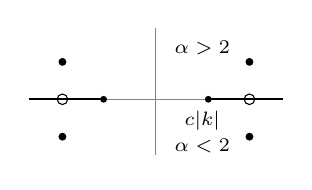
\begin{tikzpicture}[scale=0.95]
\draw[gray] (-1.7,0)--(1.7,0); \draw[gray] (0,-0.75)--(0,0.95);
\draw[thick] (-1.7,0)--(-0.7,0); \draw[thick] (0.7,0)--(1.7,0);
\fill (0.7,0) circle (1.3pt); \fill (-0.7,0) circle (1.3pt);
\draw (1.25,0) circle (2.0pt); \draw (-1.25,0) circle (2.0pt);
\fill (1.25,0.5) circle (1.5pt); \fill (-1.25,0.5) circle (1.5pt);
\fill (1.25,-0.5) circle (1.5pt); \fill (-1.25,-0.5) circle (1.5pt);
\node[font=\scriptsize] at (0.62,0.68) {$\alpha>2$};
\node[font=\scriptsize] at (0.62,-0.62) {$\alpha<2$};
\node[font=\scriptsize,anchor=north] at (0.62,-0.02) {$c|k|$};
\end{tikzpicture}\par
{\scriptsize the $\omega$ plane}
\end{minipage}\hfill
\begin{minipage}[c]{0.78\linewidth}
{\small\renewcommand{\arraystretch}{1.05}\setlength{\tabcolsep}{3pt}
\begin{tabular}{@{}l l l l l l l@{}}
\toprule
 & \textbf{profile} & \textbf{dynamics} & \textbf{state} & \textbf{equation} & \textbf{structure} & \textbf{off the order}\\
\midrule
$\alpha\to1^-$ & fixed & update $J_{n+1}=T_n$ & $J$ & Schr\"odinger & Galilean & leak $\tfrac\pi4(1-\alpha)$\\
$\alpha=2$ & radius $c\tau$ & balance $T=S$ & $(J,\partial_tJ)$ & Klein--Gordon & Lorentz & rate $\tfrac\pi4(2-\alpha)\mu^2/\omega$\\
\bottomrule
\end{tabular}}\par\vspace{2pt}
{\small The edge and the closure, the two places where the law is marginal: unitary in the limit at the edge, conservative at the closure. Each is unitary or conservative exactly at its order, and each state is kept by accumulation: one accumulator at the edge, one per null leg at the closure. Left: at $\alpha=2$ the roots $\pm\omega$ sit on the real axis (open circles); above the order they rise and the response runs away, below it they sink and decay, and the cuts from $\pm c|k|$ carry the tail.}
\end{minipage}

\vspace{3pt}\needspace{1.2in}
{\large\textbf{The path sum}}\par
\[
J=\tfrac12\sum_{n\ge0}(-\mu^2)^n\,G^{*n}*S,\qquad\sup_x\big|G^{*n}*S\big|\le\frac{(t-t_0)^{2n}}{(2n)!}\sup|S|,\qquad\sup_x|J|\le\tfrac12\cosh\big(\mu(t-t_0)\big)\sup|S|
\]
\par\vspace{3pt}\forcesline{forces the field equation to be a sum over histories}\repline{\rep{The Neumann series of the balance: a geometric series in the invariant operator $G$, with symbol $\sum(-\mu^2)^n(s^2+c^2k^2)^{-n-1}=1/(s^2+c^2k^2+\mu^2)$. It converges absolutely for every bounded source with zero past, and its sum is the only locally bounded solution. Every term is Lorentz invariant. \tg{Lean \lean{pathsum_majorant}, \lean{rl_two_factorial}, \lean{pathsum_symbol_geometric}; sympy E: Thm pathsum}}}

\[
d=3:\qquad G^{*(n+1)}(t,x)=\int\delta\Big(t-\sum_{i=0}^n\tau_i\Big)\,\delta^3\Big(x-c\sum_{i=0}^n\tau_i\hat\omega_i\Big)\prod_{i=0}^n\tau_i\,d\tau_i\,\frac{d\Omega_i}{4\pi}
\]
\par\vspace{3pt}\repline{\rep{A history is $n+1$ null legs, leg $i$ of duration $\tau_i$ in direction $\hat\omega_i\in S^2$, with weight $\tau_i$ per leg and the real amplitude $-\mu^2$ at each of the $n$ corners. Each term is the past re-entering the present $n$ times along the cone: the sum over histories is the memory series. \tg{sympy E: Thm pathsum (4)}}}

\[
d=1:\qquad G^{*(n+1)}=\frac{\theta(u)\theta(v)}{2c}\,\frac1{(n!)^2}\Big(\frac{uv}{4c^2}\Big)^{n},\qquad G_\mu=\frac{\theta(u)\theta(v)}{2c}\,J_0\Big(\mu\sqrt{t^2-x^2/c^2}\Big)
\]
\par\vspace{3pt}\repline{\rep{Each step integrates once in $u$ and once in $v$, so the $n$-th term is $u^nv^n/(n!)^2$, a function of the invariant $uv=c^2t^2-x^2$ alone; the sum is the Bessel series, and with all signs positive it is $I_0$. \tg{Lean \lean{checker_step}; sympy E: Prop checker (1); mpmath A: sums against $J_0$, $I_0$ to $10^{-40}$}}}

\[
(-\mu^2)^n\,G^{*(n+1)}=\frac{\Phi_{2n+1}}{2ic\mu},\qquad\Phi_{2n+1}=\frac{(i\mu)^{2n+1}}{(n!)^2}\Big(\frac{uv}{4c^2}\Big)^n,\qquad L_\eps=\sum_n(i\eps\mu)^{2n+1}\binom{N_R-1}{n}\binom{N_L-1}{n},\quad\frac{L_\eps}\eps\to i\mu J_0
\]
\par\vspace{3pt}\forcesline{forces Feynman's checkerboard, term by term}\repline{\rep{The law's insertion is real, $-\mu^2$ per corner of a light-cone history; Feynman's is imaginary, $i\mu$ per corner of a null zigzag. They agree because $(-\mu^2)^n=(i\mu)^{2n}$: one step of $G$ is a $u$-leg and a $v$-leg, so $n$ insertions make $2n+1$ corners, each a flip of chirality. $\Phi_{2n+1}$ is amplitude times volume in leg durations; of the divisor, $2c$ is the Jacobian to a density in $x$ and $i\mu$ one corner. One orientation of first and last step is counted. \tg{Lean \lean{neg_mu_sq_pow}, \lean{checker_factor}, \lean{checker_binomial_bound}; sympy E: brute-force corner count over all paths to $16$ steps; mpmath A: error $O(\eps)$}}}

\[
d=3:\qquad G_\mu=\frac{\delta(r-ct)}{4\pi cr}-\theta(ct-r)\,\frac{\mu}{4\pi c^2}\,\frac{J_1(\mu\sqrt w/c)}{\sqrt w},\qquad w=c^2t^2-r^2
\]
\par\vspace{3pt}\forcesline{forces the interior of the cone: the corners alone fill it}\repline{\rep{Histories without corners lie on the cone, Huygens' principle. Every history with at least one corner lands strictly inside, since $|\sum\tau_i\hat\omega_i|<\sum\tau_i$ unless all directions coincide. So the Bessel tail of the massive propagator is the sum over histories with a corner. \tg{sympy E: Prop descent3; mpmath A: against $J_1$, $I_1$ to $10^{-40}$}}}

\[
d=3,\ n\ge1:\qquad G^{*(n+1)}=\theta(ct-r)\,\frac{n\,w^{n-1}}{2\pi c\,(4c^2)^n(n!)^2},\qquad\sum_{n\ge1}\mu^{2n}\big|G^{*(n+1)}\big|=\frac{\mu}{4\pi c^2}\,\frac{I_1(\mu\sqrt w/c)}{\sqrt w}
\]
\par\vspace{3pt}\repline{\rep{Descent applied term by term: $w^n$ vanishes on the cone, so no shell term appears beyond $n=0$, and each interior term is a polynomial in the invariant $w$. The tail converges absolutely. In every dimension the terms depend on the point only through its invariant interval from the source. \tg{sympy E: Prop descent3, termwise; mpmath A: terms by direct convolution quadrature}}}

\vspace{3pt}\needspace{1.2in}
{\large\textbf{Composition, unitarity and the readout}}\par
\[
\begin{pmatrix}\hat J\\ \partial_t\hat J\end{pmatrix}(t)=M_k(t-t_1)\begin{pmatrix}\hat J\\ \partial_t\hat J\end{pmatrix}(t_1),\qquad
M_k(t)=\begin{pmatrix}\cos\omega t&\omega^{-1}\sin\omega t\\ -\omega\sin\omega t&\cos\omega t\end{pmatrix},\qquad M_k(t+t')=M_k(t)M_k(t')
\]
\par\vspace{3pt}\forcesline{forces Markov structure: the past enters through the pair}\repline{\rep{$M_k(t)$ has determinant $1$ and trace $2\cos\omega t$: a one-parameter elliptic subgroup of $SL(2,\mathbb R)$, the same class as the edge's recurrence below its order. The memory reaches over the whole past cone, yet the past enters through two accumulated quantities; no records are kept, so this is not the faithful limit. \tg{Lean \lean{Mk_add}, \lean{Mk_det}; sympy E: Prop pair; G2}}}

\[
J(t)=e^{\mp i\hat Ht/\hbar}J(0),\qquad\hat H=\sqrt{m^2c^4-\hbar^2c^2\nabla^2};\qquad Q=\int JJ^\dagger\,d^dx\ \ \text{constant on one sign of frequency}
\]
\par\vspace{3pt}\forcesline{forces one sign of frequency for the Born readout}\repline{\rep{The two sheets of the mass shell carry the two unitary representations; on one sheet the evolution is a unitary group acting on the spatial factor, so the closure, its trace and the readout $p_m=\tr(P_mQ)/\tr Q$ are constant. With both signs, $\lVert J\rVert^2$ has the cross term $2\,{\rm Re}\int\tr(a_+^\dagger a_-)e^{2i\omega t}$ and is constant only if that vanishes, as when the signs sit in different matrix entries. \tg{Lean \lean{norm_mode}, \lean{closure_const}, \lean{closure_two_modes}, \lean{mixed_mode_not_const}; sympy E: Thm unitary; numpy N: spread $7\times10^{-13}$ on one sign, $6\times10^{-4}$ mixed}}}

\[
q(J)=\frac{i\hbar}{2mc^2}\int\tr\big(J^\dagger\partial_tJ-\partial_tJ^\dagger J\big)\,d^dx,\qquad0\le q(J)-\lVert J\rVert^2\le\frac{\hbar^2}{2m^2c^2}\,\lVert\nabla J\rVert^2
\]
\par\vspace{3pt}\repline{\rep{Two positive quantities are conserved on positive frequency. $q$ is the charge of a local conserved current, the same in every inertial frame, and conserved on every solution. $\lVert J\rVert^2$ is conserved in each frame but is not the charge of a local current. They differ at order $v^2/c^2$. A frame-independent position readout is the Newton--Wigner problem and is not claimed. \tg{Lean \lean{charge_ratio_bounds}; sympy E: Thm unitary (4); numpy N: charge constant to $2\times10^{-14}$; frame dependence not checked}}}

\vspace{3pt}\needspace{1.2in}
{\large\textbf{The nonrelativistic limit}}\par
\[
\big\lVert e^{-i(\hat H-mc^2)t/\hbar}\psi-K_F(t)\psi\big\rVert\le\frac{|t|\hbar^3}{8m^3c^2}\,\lVert\Delta^2\psi\rVert,\qquad K_F(t)=e^{i\hbar t\nabla^2/2m}
\]
\par\vspace{3pt}\forcesline{forces Schr\"odinger from above, with error $O(1/c^2)$}\repline{\rep{As $c\to\infty$ the Poincar\'e group contracts to the Galilei group, and the rest phase $e^{-imc^2t/\hbar}$ that is removed is its central term. Mode by mode, $0\le\hbar^2k^2/2m-(\hbar\omega-mc^2)\le\hbar^4k^4/(8m^3c^2)$; the constant $\tfrac18$ is sharp, and the next term is $\hbar^5k^6/(16m^5c^4)$. Both evolutions are unitary for every $c$. \tg{Lean \lean{nr_dispersion_bounds}, \lean{nr_mode_bound}; sympy E: Thm NR; mpmath A: error times $c^2\to3.67151$}}}

\[
K_F(t)=\lim_{c\to\infty}\frac{2mc^2}{i\hbar}\,e^{imc^2t/\hbar}\Big[\sum_{n\ge0}(-\mu^2)^n\,G^{*(n+1)}(t)\Big]^+
\]
\par\vspace{3pt}\forcesline{forces Feynman's kernel as the Galilean limit of the light-cone path sum}\repline{\rep{The positive-frequency part of the sum over piecewise-null histories, with the rest phase removed, converges strongly to Feynman's free kernel, and time slicing is the limit of the group law. At finite $c$ the rescaled kernel is not itself a group, because of its prefactor $mc^2/\hbar\omega$; the group law belongs to $e^{-i(\hat H-mc^2)t/\hbar}$. The dynamics at $\alpha=2$ is real: $G$, $-\mu^2$ and $J_0$ are real, and the $i$ of $K_F$ enters only through the sign of frequency inherited from the source. \tg{Lean \lean{feynman_amplitude_bounds}; sympy E: Cor feynman}}}

\vspace{2pt}
\begin{smallbox}
\textbf{What the numbers say.} Exact roots, quadrature and a direct null-lattice simulation, with code independent of the paper's script.\par\vspace{2pt}
{\renewcommand{\arraystretch}{1.0}\setlength{\tabcolsep}{4pt}
\begin{tabular}[t]{@{}l c c c c c c c@{}}
\toprule
$\alpha$ & $0$ & $0.5$ & $1.5$ & $1.9$ & $2$ & $2.1$ & $3$\\
\midrule
$\max_\varphi|h_\alpha-1|$ & $0$ & $0.41$ & $0.41$ & $0.097$ & $0$ & $0.10$ & $1.0$\\
\bottomrule
\end{tabular}\hfill
\begin{tabular}[t]{@{}l c c c@{}}
\toprule
step $h$ & $0.08$ & $0.04$ & $0.02$\\
\midrule
error against KG & $7.1\times10^{-3}$ & $1.8\times10^{-3}$ & $4.4\times10^{-4}$\\
\bottomrule
\end{tabular}}\par\vspace{3pt}
{\renewcommand{\arraystretch}{1.0}\setlength{\tabcolsep}{4pt}
\begin{tabular}[t]{@{}l c c c c@{}}
\toprule
step $\eps$ & $0.02$ & $0.01$ & $0.005$ & $0.0025$\\
\midrule
$\max|L_\eps/(i\eps\mu)-J_0|$ & $3.70\times10^{-2}$ & $1.81\times10^{-2}$ & $8.95\times10^{-3}$ & $4.45\times10^{-3}$\\
\bottomrule
\end{tabular}\hfill
\begin{tabular}[t]{@{}l c c c@{}}
\toprule
$\alpha$, at $k=1$ & $1.95$ & $2.05$ & $2.10$\\
\midrule
${\rm Im}\,\omega$ & $-2.75\times10^{-2}$ & $2.79\times10^{-2}$ & $5.59\times10^{-2}$\\
\bottomrule
\end{tabular}}\par\vspace{2pt}
{\renewcommand{\arraystretch}{1.0}\setlength{\tabcolsep}{4pt}
\begin{tabular}[t]{@{}l c c c c c@{}}
\toprule
$c$ & $2$ & $4$ & $8$ & $16$ & $32$\\
\midrule
error $\times\,c^2$ & $2.423$ & $3.321$ & $3.589$ & $3.651$ & $3.667$\\
\bottomrule
\end{tabular}\hfill
\begin{tabular}[t]{@{}l c c c c@{}}
\toprule
$k$ & $0$ & $0.5$ & $1$ & $2$\\
\midrule
root $E$ & $1.000000$ & $1.118034$ & $1.414214$ & $2.236068$\\
\bottomrule
\end{tabular}}\par\vspace{2pt}
Top: the Lorentz defect vanishes only at $\alpha=0$ and $2$; the simulated law converges to Klein--Gordon at second order, and its measured $\mu\tau_c$ extrapolates to $0.7071068$. Bottom: the checkerboard converges at first order in $\eps$; the rates off $\alpha=2$. Below the order, at $\alpha=1.9$ and $k=1$, the response at $t=600$ is $1.6\times10^{-6}$ where the pole alone gives $5\times10^{-15}$: the tail. Last row: the packet $e^{-x^2/8+ix}$ at $t=10$, whose error times $c^2$ tends to $3.6712$ against the bound $3.6715$; and the roots of the balanced law, equal to $\sqrt{k^2+\mu^2}$ to ten digits. \tg{mpmath A; numpy N}
\end{smallbox}

\vspace{1pt}
\begin{smallbox}
\textbf{Remark (where the $i$ comes from).} At the edge the $i$ of the Schr\"odinger equation is the rotation produced by negative feedback on the accumulated past. At $\alpha=2$ the dynamics is real, and the $i$ of Feynman's kernel enters only through the sign of frequency, which is inherited from the source's past; nothing near $\alpha=2$ selects it. In $1+1$ dimensions it is also the corner amplitude whose square is the real insertion.\par\vspace{1pt}
\textbf{Remark (histories are memory).} Each term of the Feynman sum is the past re-entering the present $n$ times along the light cone, weighted by the order-two lag $\tau$ per leg and by $-\mu^2$ per re-entry. Its Markov form is the pair $(J,\partial_tJ)$, and its Galilean limit is Feynman's kernel. \textbf{Open:} interaction between carriers, where the return-leg structure the edge lacks is now available.
\end{smallbox}

\vspace{1pt}
\begin{smallbox}
\textbf{What the checks changed.} No constant, sign or factor in a displayed formula was wrong. These statements were repaired, and this sheet uses the repaired forms. (1) The proof of the symbol covered $\alpha>1$ only; for $0<\alpha\le1$ the formula holds by continuation in $\alpha$. (2) Near $\alpha=2$ the real part of the symbol also moves at first order, shifting the frequency; the stated rate is unaffected. (3) Below $2$ the exponential decay is followed by an algebraic tail from the light-cone branch points, which the paper did not have. (4) ``Not conserved on mixed frequencies'' is false as a universal statement: $J=E_{11}e^{-i\omega t}+E_{22}e^{i\omega t}$ has both signs and a constant closure. (5) The checkerboard amplitude is a volume in leg durations and counts one orientation. (6) The rescaled kernel is not a group at finite $c$. (7) Two table entries came from a grid edge and from a fixed first step, and one caption figure was the first-order value. \textbf{Remark (two routes to Schr\"odinger).} The edge reaches the free Schr\"odinger equation from below, Galilean from the start; the closure reaches it from above, as $c\to\infty$ opens the past cone to the whole time-ordered past. Whether the two masses coincide is not claimed; a kernel width of $\sqrt6$ Compton wavelengths at the edge would tie them. \textbf{Remark (the coframe).} Everything here is in the flat sector, where the transports are the identity. On a curved background the light-cone profile needs a frame at each point to say which directions are null and which is time, the job of a coframe; how the transports and the gauge bundle enter is deferred, as in the companion sheets.
\end{smallbox}

\vspace{1pt}
\begin{smallbox}
\textbf{Legend.} \textbf{Balance:} $T$ is the new state, and it vanishes only when the present balances the accumulated past. The edge's update rule is not used here: at $\alpha=2$ the term $2J$ alone would double the current at every update.\quad \textbf{Zero past:} $f=0$ for $t<t_0$.\quad \textbf{Light-cone width:} the profile at lag $\tau$ has radius $c\tau$; at the edge it does not depend on the lag.\quad \textbf{Positive frequency:} every Fourier mode proportional to $e^{-i\omega(k)t}$.\quad \textbf{Known:} the $1+1$ checkerboard and its nonrelativistic limit, and chain sums for the retarded propagator on causal sets. What is new is the source: the history sum is the memory series of the law at $\alpha=2$, and the light-cone width is selected by Lorentz invariance of the memory symbol.\quad \textbf{Group class notes} name the symmetry behind each row; where a note has no tag of its own it is a reading.
\end{smallbox}

\vspace{1pt}
{\large\textbf{The necessity chain}}\hfill{\footnotesize\textit{each element is forced by a modeling requirement}}\par\vspace{2pt}
{\small\renewcommand{\arraystretch}{1.0}\setlength{\tabcolsep}{3pt}\setlength{\aboverulesep}{1pt}\setlength{\belowrulesep}{1.5pt}
\begin{longtable}{@{}>{\raggedright\arraybackslash}p{1.75in}>{\raggedright\arraybackslash}p{2.25in}>{\raggedright\arraybackslash}p{1.5in}>{\raggedright\arraybackslash}p{1.75in}@{}}
\rowcolor{hdr}\textbf{Requirement} & \textbf{Structure / Element} & \textbf{Field-theory name} & \textbf{Role}\\
\midrule\endfirsthead
\rowcolor{hdr}\textbf{Requirement} & \textbf{Structure / Element} & \textbf{Field-theory name} & \textbf{Role}\\
\midrule\endhead
Causal structure must be enforced & $\nu_\tau$\ \ (light front of radius $c\tau$) & Retarded support & The memory reaches back along the cone only\\
\multicolumn{4}{@{}>{\raggedright\arraybackslash}p{7.5in}@{}}{\hspace{0.25in}\textbf{Group class.} $SO(3)$-invariant measure on a sphere; one Fourier transform in every dimension \tg{sympy E}}\\
\midrule
The memory must look the same to every observer & $\alpha=2$ & Lorentz invariance & Selects the order: the symbol is a function of $p^2$\\
\multicolumn{4}{@{}>{\raggedright\arraybackslash}p{7.5in}@{}}{\hspace{0.25in}\textbf{Group class.} Boost invariance, exactly when $h_\alpha$ is constant \tg{Lean \lean{lorentz_selects_two}}}\\
\midrule
The present must answer to the past & $T=2J+K_2J=S$\ \ (balance) & Equation of motion & Klein--Gordon wherever the source vanishes\\
\multicolumn{4}{@{}>{\raggedright\arraybackslash}p{7.5in}@{}}{\hspace{0.25in}\textbf{Group class.} The mass shell $p^2=m^2c^2$, a level set of the Poincar\'e Casimir \tg{Lean \lean{kg_dispersion}}}\\
\midrule
No external scale & $\mu\tau_c=1/\sqrt2$ & Mass & The kernel's own rate; only ratios are physical\\
\multicolumn{4}{@{}>{\raggedright\arraybackslash}p{7.5in}@{}}{\hspace{0.25in}\textbf{Group class.} Quotient by dilations: the symbol is homogeneous of degree $-2$ \tg{Lean \lean{mu_tau}}}\\
\midrule
A field must start somewhere & $S$ with zero past & Retarded boundary condition & A source is an imbalance; no initial data are used\\
\multicolumn{4}{@{}>{\raggedright\arraybackslash}p{7.5in}@{}}{\hspace{0.25in}\textbf{Group class.} Support in the forward cone, preserved by the orthochronous group; the bounded solution is unique \tg{sympy E; Lean \lean{pathsum_majorant}}}\\
\midrule
The past must re-enter & $(-\mu^2)^nG^{*n}$\ \ (Neumann series) & Mass insertions on a massless line & Sum over piecewise-null histories\\
\multicolumn{4}{@{}>{\raggedright\arraybackslash}p{7.5in}@{}}{\hspace{0.25in}\textbf{Group class.} Geometric series in an invariant operator; each term invariant \tg{Lean \lean{pathsum_majorant}}}\\
\midrule
History must fade appropriately & conservative exactly at $\alpha=2$ & Stability & Decay and a tail below, runaway above\\
\multicolumn{4}{@{}>{\raggedright\arraybackslash}p{7.5in}@{}}{\hspace{0.25in}\textbf{Group class.} Time-reversal symmetry of the symbol, at $\alpha=2$ only \tg{mpmath A; numpy N}}\\
\midrule
The phase must come from the law's own order & $\theta=\alpha\pi/2=\pi$ & Sign of the mass term & Two quarter turns; an added sign gives a tachyon\\
\multicolumn{4}{@{}>{\raggedright\arraybackslash}p{7.5in}@{}}{\hspace{0.25in}\textbf{Group class.} The half turn $e^{i\pi}=-1$ in $U(1)$, supplied by the double accumulation \tg{Lean \lean{kg_dispersion_flipped}}}\\
\midrule
Space of any dimension & $\mathcal D$\ \ (descent) & Method of descent & $1+1$ results lift to $3+1$; the corners fill the cone\\
\multicolumn{4}{@{}>{\raggedright\arraybackslash}p{7.5in}@{}}{\hspace{0.25in}\textbf{Group class.} The symbol depends on $|k|$ alone, in every dimension \tg{sympy E; mpmath A}}\\
\midrule
The state must be finite & $(J,\partial_tJ)$\ \ (the pair) & Phase space & One accumulator per null leg; no records\\
\multicolumn{4}{@{}>{\raggedright\arraybackslash}p{7.5in}@{}}{\hspace{0.25in}\textbf{Group class.} Elliptic one-parameter subgroup of $SL(2,\mathbb R)$ \tg{Lean \lean{Mk_add}; G2}}\\
\midrule
A direction of time & one sign of frequency & Particle or antiparticle sheet & Makes the trace readout a conserved norm\\
\multicolumn{4}{@{}>{\raggedright\arraybackslash}p{7.5in}@{}}{\hspace{0.25in}\textbf{Group class.} One sheet of the mass shell; inherited from the source's past, not selected by the law \tg{Lean \lean{closure_const}}}\\
\midrule
The state must be read & $Q=\int JJ^\dagger$\ \ (closure) & Born readout & Conserved and normalized in each frame\\
\multicolumn{4}{@{}>{\raggedright\arraybackslash}p{7.5in}@{}}{\hspace{0.25in}\textbf{Group class.} Invariant under the unitary group on the spatial factor; the left projectors commute with it \tg{sympy E; numpy N}}\\
\midrule
Slow carriers must look Galilean & $c\to\infty$ & Nonrelativistic limit & Feynman's free kernel, error $O(1/c^2)$\\
\multicolumn{4}{@{}>{\raggedright\arraybackslash}p{7.5in}@{}}{\hspace{0.25in}\textbf{Group class.} Contraction of the Poincar\'e group to the Galilei group \tg{Lean \lean{nr_dispersion_bounds}}}\\
\midrule
\end{longtable}}

\vspace{2pt}
{\footnotesize
\emergencystretch=3em \textbf{Machine verification.} Four independent checks of the $\alpha=2$ paper, none reusing its script. \textbf{Lean} 4.35.0 with Mathlib v4.35.0, file \texttt{FeynmanAlphaTwo.lean}: 38 theorems, no \texttt{sorry}, axioms only \texttt{propext}, \texttt{Classical.choice}, \texttt{Quot.sound}; these are algebraic cores of the tagged rows. \textbf{sympy E}: 95 exact and symbolic checks, labelled by the paper's statement; \textbf{G1--G4}: the boost on null coordinates, the class of the pair matrix, the next defect coefficient and the rotation of $(s,c|k|)$. \textbf{mpmath A}: 231 checks at 40 digits or more, one failure, the caption figure now corrected. \textbf{numpy N}: 29 checks by direct simulation, then the paper's script run unchanged, which reproduces its tables.
\textbf{Not machine-checked:} in Lean, the symbol formula itself, the Green's function, the descent, the Bessel resummations, the lattice limit of the checkerboard, the rate near $\alpha=2$ and the step from one Fourier mode to $L^2$, all checked symbolically or numerically only; the frame dependence of $\lVert J\rVert^2$; the cited results (Stone, Kirchhoff, descent, the known checkerboard limit); the field-theory names, the remarks and the untagged group class notes, which are readings.\par}
\end{document}
